\section{Component Tools for Reproducible Research}

We have constructed a first approximation of the invariant framework
by using and modifying a variety of existing technologies.  Of course,
a viable long-term strategy for reproducibility must not depend on a single
technology.
To this end, we have identified multiple technologies 
that can implement each stage of the framework.

{\bf Capturing Dependencies.}  
The Unix {\tt ptrace} mechanism
allows a tracing process to observe all of the system calls performed by
an application, inferring each of the resources upon which an application
depends.  We have extended two existing tracing tools in order to capture
dependency information at the granularity of files and directories. 
Dependency may refer to source code, if available, or a binary file.

Parrot is a virtual filesystem access tool which
is used to attach applications to a variety of remote I/O systems such as HTTP, FTP, and CernVM-FS. It works by trapping system calls through the {\tt ptrace} interface and replacing selected operations with remote accesses.  As a side-effect, Parrot is
also able to modify the filesystem namespace in arbitrary ways according to user
needs. Parrot is particularly used in the high-energy physics community
to provide remote access to application software via CernVM-FS.
To capture dependencies, we made small modifications to Parrot to record
the logical name of every file accessed by an application into an external
dependency list.  After execution is complete, a second tool is used to copy
all of the named dependencies into a package.

The second tool, PTU~\cite{pham2014framework}, is designed to create a package of an application by recording all of the binaries, libraries, scripts, data files, and environment variables used by a program.   PTU uses the lightweight virtualization software tool Code Data Environment (CDE) to observe system calls, but takes a snapshot of every file at the point of access. In addition to files, PTU records \emph{metadata} about the execution environment, such as Linux kernel version, application version, and dynamic library versions by using standard Unix commands.  PTU also records \emph{provenance} in the form of a graph that describes how each file is created or consumed by processes within the application.  Because PTU is focused solely on the problem of preservation, it can achieve lower overhead than Parrot when remote data access is not a requirement, as we show below.

{\bf Preservation of Dependencies.}  Both Parrot and PTU can observe the precise
set of files accessed by an application.  If this precise list of files is preserved
then it should be possible to execute
\emph{exactly} the same application on \emph{exactly} the same inputs a second
time.  However, if the objective is to \emph{re-purpose} the application by running it in slightly different configurations, then the preserved package may need to
be more comprehensive than the strict dependency list.

Many possible heuristics exist for creating the preserved package
from the dependency list.  We have implemented three:
In a {\bf shallow copy}, we copy only
the exact dependencies.  Where a directory was listed, a directory is created and populated with empty files as placeholders to facilitate a directory listing.  In a {\bf medium copy}, every file in every directory mentioned by the application is preserved one level deep.  In a {\bf deep copy}, every file in every directory mentioned by the application is copied recursively.  Obviously, the more aggressive the preservation, the larger the package, but also the greater the possibility that the package can be adapted to other uses.  Other approaches to package generation might including generating the union
of multiple dependency sets, or allowing an expert user to manually add
and remove dependencies.

Both Parrot and PTU generate packages that consist of plain filesystem trees representing the namespace and data of the preserved application, and can be easily transformed into whatever archive format (e.g. ZIP or TGZ) is most suitable.  This is desirable for long-term preservation that may outlive various deployment technologies.
However, neither technology yet integrates the programming environment envisioned above for the documentation purpose.  Without these techniques, the preserved packages will have diminishing value over time.

{\bf Distribution and Deployment.} Once generated, application packages must be collected, curated, and made
available through publicly shared repositories.  Currently, a 
wide variety of services and efforts exist in order to share binary objects in this way,
and so we assume such multiple services will be available in the future.

Of more immediate interest is the ability to deploy a preserved
package at a desired execution site.  Again, long-term preservation
requires artifacts that are independent of any particular technology,
so the package must be sufficiently self-describing in order
to work with multiple technologies.  The packages produced by both Parrot and PTU
can today be re-executed through any of the following mechanisms:

(1) Re-running the application through Parrot, which can dynamically construct
the desired namespace and limit file accesses to within the preserved package.
(2) Generating a virtual machine image from the package, which can be loaded
into a local virtual machine monitor, or transferred to a cloud service provider.
(3) Converting the package into a Docker image format, enabling it to be
deployed within a lightweight Linux container.

 % Docker images
\vspace{5pt}
\noindent{\bf Linux Containers and Docker Images.} 
Linux Containers provide multiple isolated instances of execution on top of the same kernel through OS-level virtualization. Thus they can be used to persist the captured packages into images. Using such containers, Docker now allows for the preservation of the image in a more user-friendly way. Docker also provides portable deployment of containers across platforms, documentation of packages in a scriptable format, and versioning of container images. The image can be preserved along with \em{dockerfiles}, which are text files containing all the commands to build a Docker image. Similar to shell scripts, the computational section can help other provisioning tools (e.g. Chef, Puppet).  The text section, written for human consumption, is more suited for use with a version management system such as subversion or git, which can track any changes made to the dockerfile. Thus dockerfiles can be used to preserve the namelist of Parrot packages and provenance description in PTU. Docker is integrated with a continuous build environment that will not only check and validate the version of the software in present use, but also make use of a more recent version to build application software.

\begin{figure*}
\centering
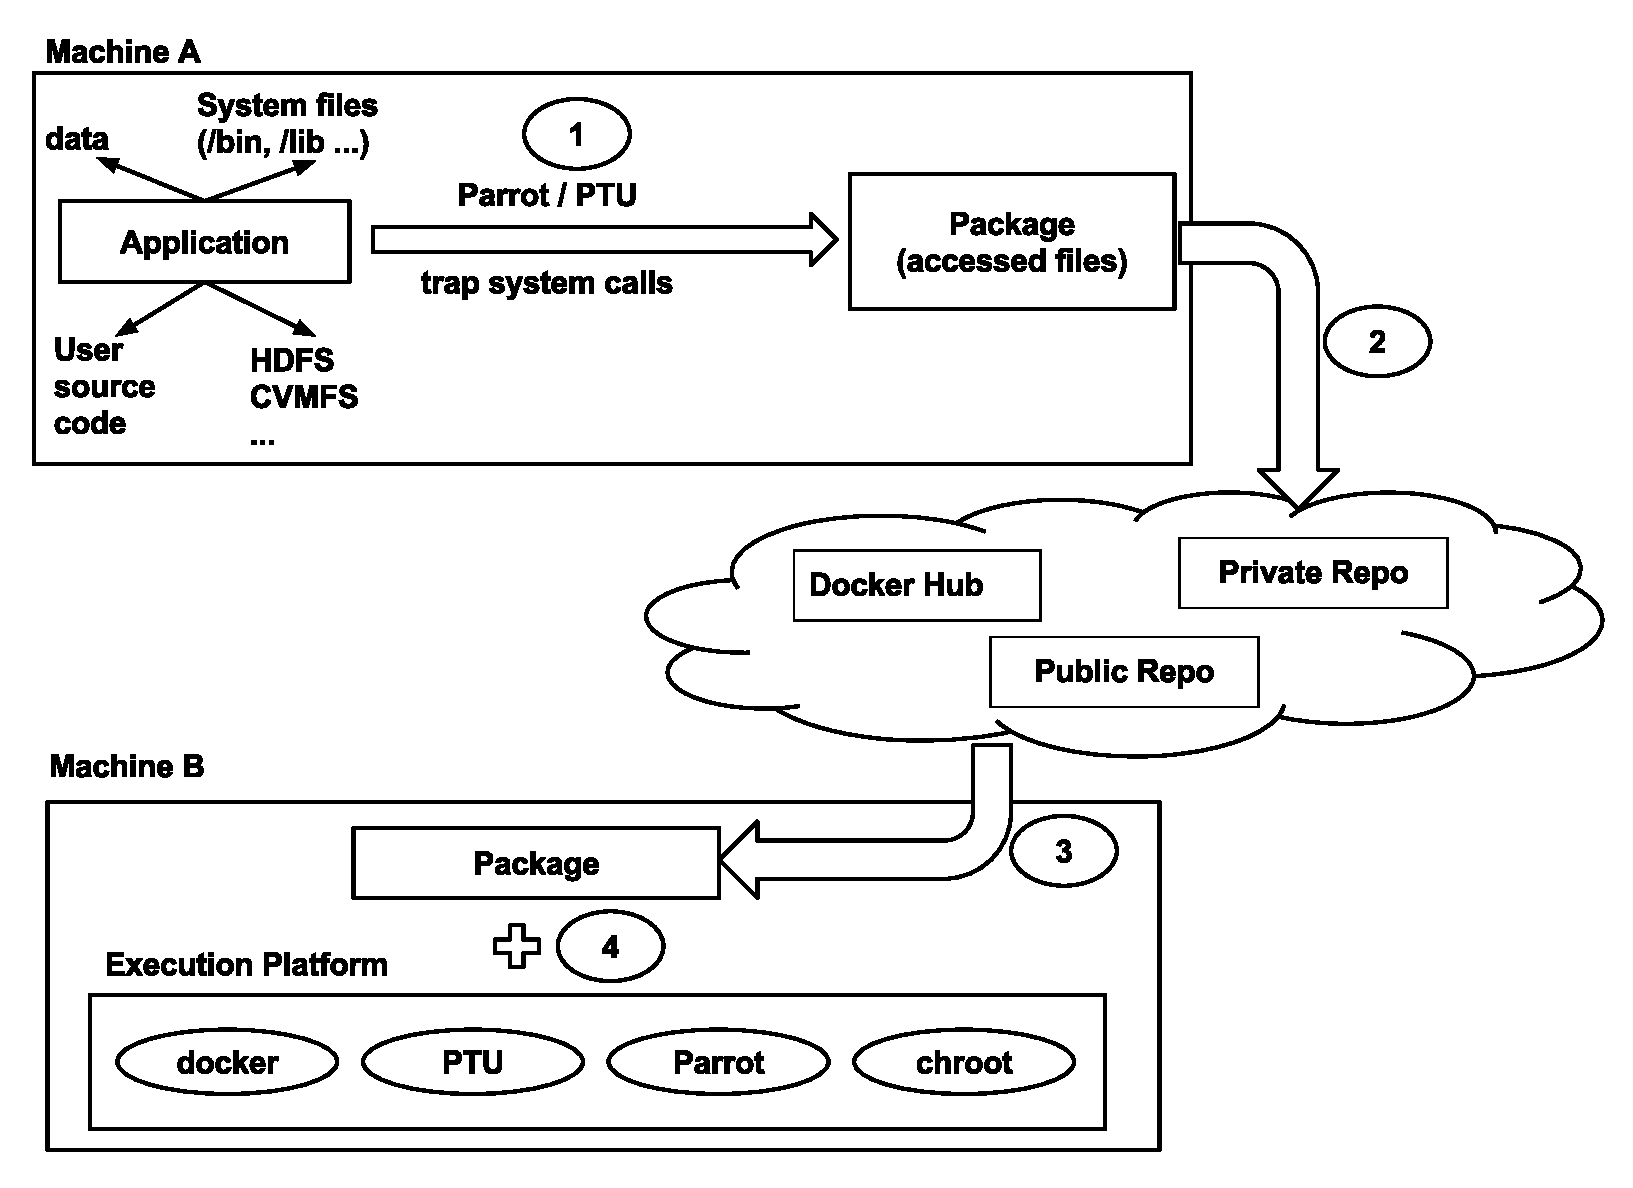
\includegraphics[width=1.0\textwidth]{preservation_framework.eps}
\caption{Preservation Framework}
\label{fig: preservation_framework}
\end{figure*}

